%-----------------------------------------------------------------------------
%
%               Template for sigplanconf LaTeX Class
%
% Name:         sigplanconf-template.tex
%
% Purpose:      A template for sigplanconf.cls, which is a LaTeX 2e class
%               file for SIGPLAN conference proceedings.
%
% Guide:        Refer to "Author's Guide to the ACM SIGPLAN Class,"
%               sigplanconf-guide.pdf
%
% Author:       Paul C. Anagnostopoulos
%               Windfall Software
%               978 371-2316
%               paul@windfall.com
%
% Created:      15 February 2005
%
%-----------------------------------------------------------------------------


\documentclass[10pt,numbers,preprint,nocopyrightspace]{sigplanconf}

% The following \documentclass options may be useful:

% preprint      Remove this option only once the paper is in final form.
% 10pt          To set in 10-point type instead of 9-point.
% 11pt          To set in 11-point type instead of 9-point.
% numbers       To obtain numeric citation style instead of author/year.

\newif\iffull
\fullfalse

\usepackage{times}
\usepackage{graphicx}
\usepackage{mathtools}
\usepackage{amsmath}
\usepackage[utf8]{inputenc}
\usepackage{cleveref}
\usepackage{listings}
\usepackage{array}
\usepackage{breqn}
\usepackage{tikz}
\usepackage{algorithmicx}
\usepackage[Algorithm,ruled]{algorithm}
\usepackage{algpseudocode}
\usepackage{pifont,xspace}
\usetikzlibrary{automata,positioning}
\newcommand{\name}{Genesis\xspace}
\newcommand{\Name}{\name}
\newcommand{\pushcode}[1][1]{\hskip\dimexpr#1\algorithmicindent\relax}
\newcolumntype{P}[1]{>{\centering\arraybackslash}p{#1}}

\usepackage[font=small]{caption}
\usepackage{enumitem}
%\usepackage{usenix}
\usepackage{epsfig}
%\usepackage[TABBOTCAP]{subfigure}
\usepackage{color}
%\usepackage{thumbpdf}
\usepackage{verbatim}
%\usepackage{hyperref}
\usepackage{url}
%\usepackage{booktabs}
\usepackage{colortbl}
\usepackage{enumitem}
\usepackage[export]{adjustbox}
\usepackage{subfig}
\usepackage{mathtools}
\usepackage{amsthm}
\usepackage{multirow}% http://ctan.org/pkg/multirow
\usepackage{hhline}
\newcommand{\minisection}[1]{\smallskip\noindent{\bf #1.}}
\newcommand{\secref}[1]{{\S\ref{#1}}}
\newcommand{\secsref}[2]{{Sections~\ref{#1} and \S\ref{#2}}}
\newcommand{\figsref}[2]{{Figure~\ref{#1} and \ref{#2}}}
\newcommand{\appref}[1]{{Appendix~\ref{#1}}}
\newcommand{\thmref}[1]{{Theorem~\ref{#1}}}
\newcommand{\lemref}[1]{{Lemma~\ref{#1}}}
\newcommand{\corref}[1]{{Corollary~\ref{#1}}}
\newcommand{\proref}[1]{{Property~\ref{#1}}}

\newcommand{\compactcaption}[1]{\vspace{-1em}\caption{#1}\vspace{-1em}}
\newcommand{\botcompactcaption}[1]{\caption{#1}\vspace{-1em}}
\newcommand{\topcompactcaption}[1]{\vspace{-1em}\caption{#1}\vspace{-0.5em}}

\newenvironment{compactitemize}
{
   \begin{itemize}[leftmargin=1.5em]
   \vspace{-1ex}
   \setlength{\topsep}{0pt}
   \setlength{\itemsep}{0em}
   \setlength{\parskip}{0pt}
   \setlength{\parsep}{0pt}
}
{
   \vspace{-1ex}
   \end{itemize}
}
\newenvironment{compact2itemize}
{
	\begin{itemize}[leftmargin=1.5em]
		\vspace{-1ex}
		\setlength{\topsep}{0pt}
		\setlength{\itemsep}{0.5em}
		\setlength{\parskip}{0pt}
		\setlength{\parsep}{0pt}
	}
	{
		\vspace{-1ex}
	\end{itemize}
}


\newenvironment{compactenumerate}
{
   \begin{enumerate}[leftmargin=1.5em]
   \vspace{-1ex}
   \setlength{\topsep}{0pt}
   \setlength{\itemsep}{0em}
   \setlength{\parskip}{0pt}
   \setlength{\parsep}{0pt}
}
{
   \vspace{-1ex}
   \end{enumerate}
}

\ifdefined\commentenabled
    \newcommand{\loris}[1]{\textcolor[rgb]{0.00,0.00,1.00}{L: #1}}
    \newcommand{\aditya}[1]{\textcolor[rgb]{0.00,0.00,1.00}{A:#1}}
    \newcommand{\kausik}[1]{\textcolor[rgb]{0.2,0.80,0.2}{K: #1}}
    \newcommand{\aaron}[1]{\textcolor[rgb]{0.00,0.2,0.6}{AGJ: #1}}
\else
    \newcommand{\loris}[1]{}
    \newcommand{\aditya}[1]{}
    \newcommand{\kausik}[1]{}
    \newcommand{\aaron}[1]{}
\fi

\newcommand{\ARC}{ARC\xspace}
\newcommand{\ARCs}{ARCs\xspace}

%\usepackage[small,compact]{titlesec}
%\usepackage[font={bf,small}]{caption}
\usepackage{titlesec}
%\titlespacing*{\section}{1pt}{3pt}{3pt}
%\titlespacing*{\subsection}{1pt}{3pt}{1.5pt}
%\titlespacing*{\subsubsection}{1pt}{3pt}{2pt}
\newtheorem{mydef}{Definition}
\newtheorem{example}{Example}
\newtheorem{theorem}{Theorem}[section]
\lstset{
	basicstyle=\itshape,
	xleftmargin=2em,
	literate={->}{$\rightarrow$}{2}
	{α}{$\alpha$}{1}
	{δ}{$\delta$}{1}
}


\crefname{Section}{§}{§§}
\Crefname{Section}{§}{§§}


\usepackage{color}
\newcommand{\loris}[1]{\textcolor[rgb]{0.00,0.00,1.00}{L: #1}}
\newcommand{\aditya}[1]{\textcolor[rgb]{0.00,0.00,1.00}{A:#1}}
\newcommand{\kausik}[1]{\textcolor[rgb]{0.00,1.00,0.00}{K: #1}}
%\renewcommand{\aditya}[1]{{\color{red}{\bf AA: #1}}}

\usepackage{float}

\newcommand{\cL}{{\cal L}}

\begin{document}

%\special{papersize=8.5in,11in}
%\setlength{\pdfpageheight}{\paperheight}
%\setlength{\pdfpagewidth}{\paperwidth}
%
%\conferenceinfo{CONF 'yy}{Month d--d, 20yy, City, ST, Country}
%\copyrightyear{20yy}
%\copyrightdata{978-1-nnnn-nnnn-n/yy/mm}
%\copyrightdoi{nnnnnnn.nnnnnnn}

% Uncomment the publication rights you want to use.
%\publicationrights{transferred}
%\publicationrights{licensed}     % this is the default
%\publicationrights{author-pays}

%\titlebanner{}        % These are ignored unless
%\preprintfooter{}   % 'preprint' option specified.

\title{Synthesizing Router Configuration based on Paths}

\authorinfo{Omitted for double blind}
{...}
{...}

\maketitle

\section{Introduction}
%% Conventionally, a network primarily acted as a backbone for
%% communication among machines, and these communications used the
%% ``shortest" path in the network based on certain metrics for deciding
%% the path between two machines.  Today,

Many enterprises are increasingly migrating their on-premise IT
infrastructure to cloud datacenters. In such environments, the
different enterprises (tenants) share different resources, such as,
the compute machines that run their applications and network
infrastructure used for communication among these applications.
Operators of such multi-tenant datacenters thus have to deal with a
multitude of machines communicating with each other (flows) over a
network that is composed of many tens to hundreds of routers or
switches (devices)~\cite{mpa-imc15}. With growing diversity of
enterprise applications and the need for security and compliance,
these pathways of communication through the datacenter network are
subject to increasingly complex network-based policies.

Consider an enterprise tenant in such a datacenter. She may desire
basic communication among her applications along shortest paths based
on certain metrics (reachability). In addition, she may wish that
traffic attempting to reach some of her applications be examined by a
set of ``middleboxes'' for auditing and access control
(traversal). Another tenant may additionally desire a subset of her
flows not share any infrastructure with others' flows for strong
security or Quality-of-Service considerations (isolation).  In
parallel, cloud operators must meet key operational objectives. For
instance, they often need to optimize network performance objectives
(traffic engineering), e.g., minimizing the maximum load imposed by
all tenants on network links, and deal with resource constraints such
as link capacity bounds and switch table sizes. Also, since datacenter
networks are highly prone to link/switch
failures~\cite{datacenterfailures}, operators need to gracefully
transition the old (pre-failure) dataplane to a policy-compliant new
(post-failure) one in a rapid and/or efficient manner.

Today, configuring network devices to implement these complex policies
and objectives in aggregate is manual, ad-hoc, and error-prone.  This
can lead to misconfigurations and violations of tenant service-level
agreements (SLAs) which can have a severe performance and security
impact.

%%  However, in real-life, the
%% process of policy enforcement by network operators is manual and
%% ad-hoc, leading to violations of service-level agreements and
%% mis-configurations which have severe performance and security
%% impacts. With the boom in cloud services, datacenter networks deal
%% with thousands of flows which are not constant, but in flux, thus,
%% making it difficult to enforce them in an ad-hoc manner.

%% Network operators desire various different end-to-end policies to
%% support in clouds and enterprise networks. Tenants or organisations
%% require support for basic policies like reachability between hosts,
%% and specifying different middlebox policies for certain
%% flows. Operators, on top of that require support for complex policies
%% like traffic isolation between flows to provide fairness and
%% specifying resource constraints like link bandwidth and switch table
%% sizes to perform traffic engineering and network resource management.

The rise of \emph{software-defined networking} (SDN) has allowed
operators to program networks in a more intuitive manner. In SDN, a
general-purpose centralized controller machine (control plane)
controls end-to-end communication pathways by managing network
forwarding rules on a collection of programmable switches (data
plane). Using a global view of current network topology, the
controller can program forwarding rules on switches based on
application requirements.
%However, many existing SDN
%frameworks are too low-level, 
%making it challenging 
%to write controller applications using these which generate 
% the data plane enforcing the above policies. %% For many
%% of the policies, generating the data plane is an NP-complete problem
%% and requires the design of efficient custom heuristics; combining
%% different policies' heuristics together is non-trivial.
Unfortunately, existing SDN programming languages (e.g.,
Frenetic~\cite{frenetic} and Pyretic~\cite{pyretic}) are too
constraining: operators would ideally want to specify and realize
policies/objectives network-wide, whereas these languages focus on programming
{\em individual} switch behaviors.  Moreover, for many types of
policies, generating a data plane that enforces them is a
%  an NP-complete 
computationally hard problem, requiring the design of efficient custom
heuristics {\em per policy/objective type}. Other recent works on
network-wide policy enforcement~\cite{merlin,simple} go beyond the
single-switch model, but they target specific types of policies/objectives and
thus are difficult to extend to other commonly desired policy types
(e.g., isolation).
%; combining  different policies' heuristics together is non-trivial. 
 %% \aditya{we need to be
% careful
%%   not to bin all SDN languages into this switch-by-switch model}
%% \kausik{Do you want to make changes here?}







%% support
%% other kinds of policies such as traffic isolation.

%%  like
%% joint bandwidth provisioning and waypoint routing in Merlin
%% \cite{merlin}, and middlebox policy enforcement in SIMPLE
%% \cite{simple} or FlowTags~\cite{flowtags}. However, these approaches

In this paper, we seek a {\em general} approach that allows a variety
of rich policies/objectives to be specified as the input, with the output being
the corresponding set of switch forwarding rules such that the
complexities of correctly realizing the policies in the data plane are
hidden from operators. This is an important step toward {\em
  intent-based networking}~\cite{intent}, where operators specify {\em
  what} they want the network to do instead of worrying about {\em
  how} the network must be configured.
%their networks. %% To support a cornucopia of policies, an
%% important feature is \emph{generality} of the approach of policy
%% enforcement, so that it can be extended to enforce custom policies
%% required by the operator.
This paper makes a case for using \emph{data plane synthesis} as a
practical approach to realizing this vision in the multi-tenant
datacenter context.
%% switch
%% table forwarding rules to the solve the problem of policy enforcement
%% by use of off-the-shelf SMT-solvers.

We present \Name, a framework for {\em declaratively} specifying and
enforcing complex policies and objectives such as, isolation,
middlebox traversals and failure resilience. To tackle the high
complexity of enforcing some of these policies (for e.g., enforcing
isolation is NP-complete), \Name encodes the problem as that of
constraint solving and leverages recent advances in fast
Satisfiability Modulo Theories (SMT) solvers to efficiently search for
a solution to the constraints.  The solution is then translated into
switch forwarding rules.
%Using SMT solvers with 
%support for linear optimization, \name can perform traffic engineering, and
%minimal network repair. We extend \name to synthesize
%resilient switch tables to \emph{proactively} ensure policy-compliance
%in failure scenarios. 
%% This
%% paper presents Genesis, a
%% network management tool where the network operators can express the
%% network-wide policies in a high-level declarative manner and Genesis
%% will synthesize the lower-level switch forwarding rules for realising
%% these policies, eliminating the need for operators to work on
%% switch-level behaviours. 
By leveraging the formal guarantees of constraint solving, \Name
eliminates the room for error in the enforcement of complex
policies and objectives.

%\kausik{Do we need to make the point of sacrificing performance for generality for POPL? }

Unfortunately, due to the the large space of forwarding plane
configurations, naively encoding policies using SMT solvers results in
slow synthesis speeds (up to hundreds-thousands of seconds in the
median case; \secref{sec:baselineeval}) which can be impractical.
%enterprise networks today because the space of forwarding plane configurations
%is huge. 
To make synthesis more practical, \Name leverages domain-specific
properties to simplify the constraints handled by the SMT solver.
We allow the network operator to write restricted
forms of regular expressions, called \emph{tactics}, that blacklist
paths based on certain patterns that are not desired in a datacenter
network.
%\loris{how about: ...based on path patterns that are not desired...}
These tactics are used to discard several constraints, 
acting as a search strategy for the solver.
%\aditya{the previous sentence is vague}
%By identifying a restricted syntax for specifying
%tactics, we 
Tactics can improve the synthesis procedure and achieve
%constraints added to the solver without additional constraints
%required to ensure the solution satisfies the tactic and achieve
a 1.5$\times - $400$\times$ speedup 
(median speedup: 1.6$\times$, average speedup: 22$\times$).

 Secondly, we develop a \emph{divide-and-conquer} synthesis procedure
 that leverages the relationships among  isolation policies to
 improve synthesis performance. The procedure partitions the input
 policies into effective components such that \name can synthesize
 these components separately and faster than the complete problem.
 Divide-and-conquer synthesis can halve the synthesis time for 40\% of
 synthetic isolation workloads.
 %% which vary in size and complexity
 %% of isolation.
 %\aditya{is this statement correct? what is 40\% of scenarios?}
 %\aditya{the
   %previous sentence is vague} 

%% are
%% huge, and by supporting a set of diverse and complex policies with
%% different search objectives, we require to create a model general and
%% expressive enough to support these. This poses a challenge as to can
%% synthesis performance be improved by leveraging knowledge specific to
%% the problem of policy enforcement in networks?

%We implement \Name using ... We evaluate it using .... Key highlights .... \aditya{all of these are todo}.\kausik{Do we need a para or will the next para suffice?}
\noindent \textbf{Contributions.} \ \ \ Our contributions are the following.
\begin{compactitemize}
\item An extensible declarative framework for describing
  complex policies/objectives and a modular SMT-based algorithm for enforcing policies and objectives
  like isolation, waypoints (\secref{sec:synthesisalgo}), traffic engineering~(\secref{sec:optimization}), and 
  failure resiliency (\secref{sec:resiliency});
\item A modified synthesis algorithm based on tactics, which leverages datacenter network structure
  to blacklist undesirable path patterns (\secref{sec:tactic});
\item A divide-and-conquer procedure for speeding up synthesis by leveraging the 
structure of policy interactions (\secref{sec:optimistic});
\item An implementation of \Name and an extensive evaluation on
  different policy/objective workloads, topologies and multi-tenancy
  settings (\secref{sec:evaluation}).
		%to quantify the performance of Genesis. 
\end{compactitemize}
%\aditya{todo}

\iffull\else
A long version
of this paper containing all the proofs has been submitted as supplementary material.
\fi
%% : We present the design and implementation of a network management
%% system with support for a diverse set of complex end-to-end
%% policies like isolation, waypoints and capacity. We designed a
%% novel search strategy using regular expressions to prune the space
%% of forwarding plane configurations by leveraging the network
%% structure to provide properties of the path, especially in
%% datacenter topologies. Lastly, we design a heuristical synthesis
%% routine leveraging the nature of policy interactions to improve
%% synthesis performance.

\section{Background}
\subsection{OSPF}

\subsection{BGP}
BGP is a path-vector routing protocol that connects 
different autonomous systems (ASes), where each AS
comprises of one or more routers (typically managed
by a single entity). 
\minisection{eBGP}
\\
\minisection{iBGP}

\subsection{BGP Best Path Selection Algorithm}
A BGP router receives multiple paths to the destination: (1)
external routes from border routers of neighbouring domains using
eBGP, and (2) routes learned by other BGP routers 
of the domain which are advertised using iBGP. 
BGP decides the best path to install in the 
forwarding table based on different metrics like local preferences,
AS path lengths and type of routes~\cite{bgp}. BGP uses the
rules specified in \Cref{alg:bgppathrules}\footnote{
For ease of presentation, we specify an abridged ruleset; 
the synthesized configurations will not use the other rules. 
} 
in decreasing order of preference to select the best path
from the received announcements. If all paths result in a tie
at $i^{th}$ rule, then the $i+1^{th}$ rule is considered.
\begin{algorithm}
	\begin{footnotesize}
		\caption{BGP Best Path Selection Rules}
		\label{alg:bgppathrules}
		\begin{algorithmic}[1]
				\State{Prefer the path with the highest \emph{local preference}.}
				\State{ Prefer the path with the smallest AS Path length. }
				\State{Prefer the path with the lowest \emph{multi-exit discriminator} (MED).}
				\State{Prefer eBGP over iBGP paths.}
				\State{Prefer the route that comes from the BGP router with the lowest \emph{router ID}.}
		\end{algorithmic}
	\end{footnotesize}
\end{algorithm}



\section{Synthesis Algorithm} \label{sec:synthesisalgo}
Given a set of policies, \Name creates constraints 
that abstract the forwarding and reachability rules such that the paths
satisfy the input policies.  
These constraints are then given to an SMT Solver, which returns a model 
for them--i.e., it assigns values to all the variables in the constraints. From these values, we extract the forwarding rules for each switch.
To provide support for the policies in \Cref{tab:policysupport}, \name uses propositional logic (SAT), linear rational arithmetic (LRA),
and linear optimization objectives for traffic engineering.
\subsection{Network Forwarding Model} \label{sec:fwdmodel}
We define the physical switch topology as an undirected graph $T=(S, L)$,
where $S$ is the set of switches and $L$ is the set of links. 
We use the neighbour function $N(s) = \{s'\ | \ (s,s') \in L \}$ to denote 
the set of neighbour switches of $s$. 
We define a set of packet classes $PC : [0,\lambda]$ and map each reachability/waypoint policy to a unique integer in $PC$.
The set of reachability policies is denoted as $R$ and each reachability policy $r \in R$ is
a pair
$(predicate :\newline src >> W_1;W_2; \ldots W_n >> dst, pc)$
where:
\begin{compactitemize}
\item  $predicate$ is the packet header identifier pertaining to $r$;
\item  $src,dst \in S$ are the source and destination switches;
\item $W_1, W_2, \ldots, W_n \subseteq S$ are the (potentially empty) ordered sets of waypoints; 
\item $pc \in PC$ is the packet class and is a unique integer used to identify the variables associated to $r$
\end{compactitemize} 
In the rest of the paper, we often use the term packet class to identify the corresponding reachability/waypoint policy. 
Other policies are not mapped to packet classes as they do not produce a path, but specify restrictions on paths of packet classes. 
%Assuming that the intersection of predicates is empty for policies in $R$, we create a mapping $\gamma : R \rightarrow PC$ to associate each reachability policy with a unique integer called packet class in the set $PC$. Switches $src, dst \in S$ denote the ingress and egress switches respectively for the packet class $pc = \gamma(r)$ and Genesis finds a path from $src$ to $dst$ for $pc$. If a waypoint policy is specified, $W$ is the set of switches the path from $src$ to $dst$ must traverse through in no particular order.
We define a static integer $\mu$ to be the synthetic limit for path length for any packet class, and define the set $K = [0, \mu]$ to be the set of all permissible path lengths.

The key roles of the network forwarding model are abstracting the actual forwarding rules at each node and encoding the reachability of each flow. 
\begin{mydef}
\label{def:fwd}
The relation $Fwd \subseteq S \times S \times PC $ captures network forwarding behavior, i.e. 
$(sw_1, sw_2$, $pc)\in$ $Fwd$ if 
$sw_1$ forwards packets of class $pc$ to switch $sw_2$. 
\end{mydef}
\begin{mydef}
\label{def:reach}
	The relation $Reach \subseteq S \times PC \times K$ captures the path reachability,
	i.e. $(sw, pc, k)\in Reach$ if 
	the switch $sw$ is reachable in the path from source switch of packet class $pc$ in exactly $k$ steps.  
\end{mydef}
For brevity, we write $Fwd(sw_1, sw_2, pc)$ for $(sw_1, sw_2, pc) $ $\in Fwd$ and similarly for the $Reach$ relation. 
Since $Fwd$ depends on the topology,
for all $sw_1, sw_2$ that are not connected by a link, 
we have that $\forall pc$, $(sw_1,sw_2,pc) \notin Fwd$. 
\begin{mydef}
	Given the set of constraints $\Psi$ generated by the synthesis algorithm from the input policies,
	$(Fwd,Reach) \models \Psi$ if $Fwd$ and $Reach$ is a model of $\Psi$.
\end{mydef}

\begin{mydef} \label{def:Pi}
Given two concrete relations $Fwd$ and $Reach$, 
the set of induced paths $\Pi = \texttt{paths}(Fwd, Reach)$ is defined as follows:
given a class $pc$,  $(sw_0 \ldots sw_k, pc) \in \Pi$ iff : 
\begin{compactenumerate}
	\item $\forall i \in [0,k]. (sw_i, pc, i) \in Reach$
	\item $\forall i \in [0, k - 1]. (sw_i, sw_{i+1}, pc) \in Fwd$
\end{compactenumerate}
\end{mydef}
\noindent Figure~\ref{fig:model} illustrates these definitions.

\begin{figure}
	\centering
	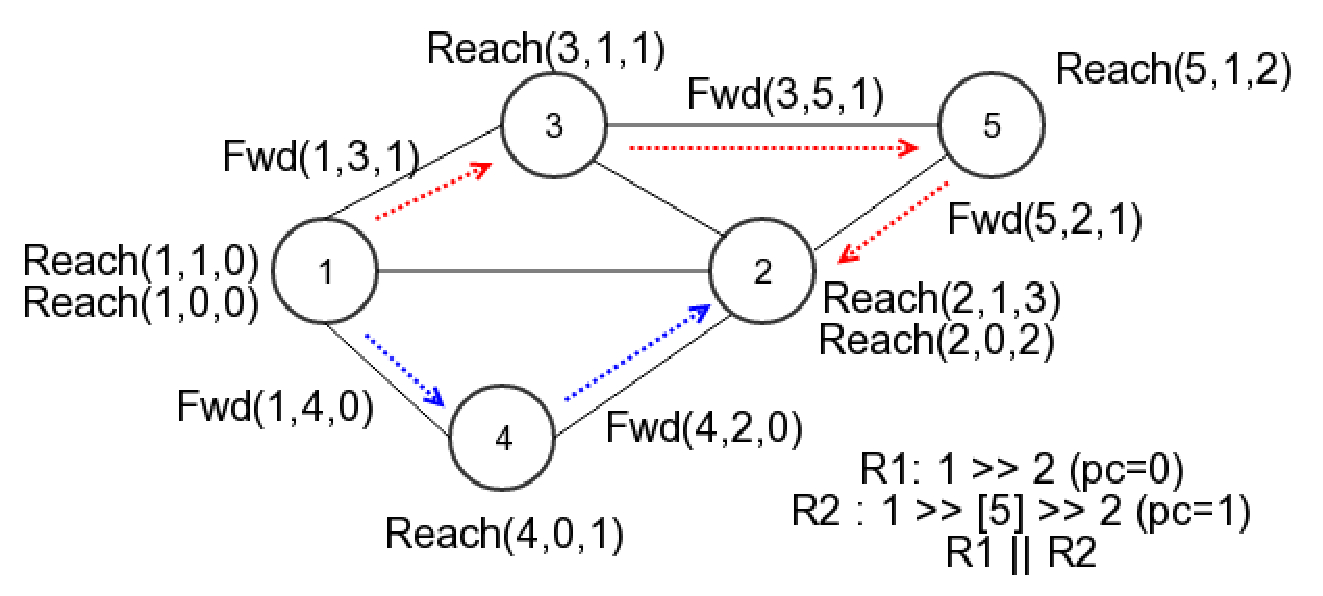
\includegraphics[width=0.8\columnwidth]{figures/network-model-example.eps}
	\caption{Values of the $Fwd$ and $Reach$ relations of the network forwarding model
		 for the policies specified in the figure. The blue and red arrows indicate the 
		 paths of packet classes 0 and 1 respectively according to the model.}
	\label{fig:model}
\end{figure}

\begin{mydef}
Given the set of constraints $\Psi$ corresponding to the input policies,
a set of paths $\Pi$ is a solution to $\Psi$, $\Pi \models \Psi$, 
if there exists $Fwd, Reach$ such that $(Fwd, Reach) \models \Psi$ and $\ \Pi=\texttt{paths}(Fwd,Reach)$.

\end{mydef}
%An example network forwarding model is shown in \cref{fig:model}. 
%%There are two reachability policies, $r1 : 1 >> [5] >> 2$ with $pc=1$ and $r2 : 1 >> 2$ with $pc=2$ and $r1$ is isolated to $r2$
%Using the value of $Fwd$ relation, we can find out paths for each packet class the forwarding rules for each switch. 

One of the decisions oriented towards performance is modelling the forwarding and reachability relations using propositions, so that we can reduce enforcement of policies like reachability, waypoints and isolation to a Boolean Satisfiability Problem (SAT) problem\footnote{An earlier iteration of our model used \emph{uninterpreted functions} and modeled reachability using recursive constraints, 
	which was slower with a greater number of constraints.}. 
The relations for forwarding and reachability ensure we can write the constraints in a concise and intuitive manner.

\subsection{Reachability Constraints} \label{sec:reach}
We first discuss the constraints generated for reachability policies without waypoints.
For a reachability policy $s >> d$ and packet class $pc$, the added constraints must ensure that 
the solution model represents a path 
from source to destination. 
The base constraint states that $(s, pc,0) \in Reach$ meaning
that $s$ can be reached in $0$ steps. 
The following constraint states that there must be a forwarding rule from $s$ to one of
the neighbors of $s$\footnote{
	We unroll the existential quantifier $\exists n \in N(s)$ using disjunction of 
	clauses $\bigvee\limits_{n \in N(s)}$ and
	the universal quantifier $\forall n \in N(dst)$ using conjunction of clauses $\bigwedge\limits_{n \in N(dst)}$
	and stay in propositional logic.}.
\begin{equation} \label{eq:src}
	\exists n \in N(s).~Fwd(s, n, pc) \wedge Reach(n, pc, 1).
\end{equation}
Next, we add the following constraints to state that $d$ can be reached in some number of steps and,
since $d$ is the last switch in the path, there are no forwarding rules from it.
\begin{equation} \label{eq:dst}
	\exists k.~Reach(d, pc, k) \ \wedge \ \forall n \in N(d). \ \neg Fwd(d, n, pc).
\end{equation}
Finally, we add implication constraints that propagate reachability backward from destination to source. 
If a node $n_1$ is reachable in $k$ steps, there must be a node $n_2$ reachable in  $k-1$ steps and 
a forwarding rule $n_2 \rightarrow n_1$.
\begin{multline} \label{eq:bckprop}
\forall n_1,k.~ Reach(n_1,pc,k) \implies \exists n_2.  n_2 \in N(n_1) \wedge \\ Reach(n_2,pc,k-1) \wedge Fwd(n_2,n_1,pc).
\end{multline} 
When combined together, these constraints %can only be satisfied if there is a valid path from $s$ to $d$.
% to destination by using the unit clauses in \cref{eq:dst}, and finding a path from destination back to a switch $sw$ which is a neighbour of $src$. $Reach(sw,pc,1)$ would be true from \cref{eq:src} and the reachability policy would be satisfied. 
are sufficient to ensure the existence of a path from $s$ to $d$ for packet class $pc$.
% in terms of the forwarding relation $Fwd$. 
However, since there is no restriction on number of $Fwd$ values that can be true at a switch, we can get multiple forwarding rules at switches, and 
also multiple paths to the destination. 
These can also create forwarding loops. 
Concretely, this is not a problem: as long as there is  at least one path from $s$ to $d$ we can recover it from the solution of the constraints. 
Moreover, this representation is quite efficient, as forcing a singular path would
require to add further constraints.
% we are able to extract a path from the solution without 
%adding additional constraints to ensure the semantics of \emph{unicast} forwarding. 

To extract a concrete $s$-to-$d$ path we 
perform a breadth-first search on the reachability graph induced by the solution to the constraints. 
A directed edge $n_1 \rightarrow n_2$ appears in the reachability-graph if there is forwarding rule indicated by the relation $(n_1,n_2, pc) \in Fwd$. 
We extract the rules relevant to the shortest path from source to destination from the model, and the additional rules obtained in the solution (extra paths, forwarding loops) are ignored.  

\subsection{Waypoint Constraints} 
For a reachability policy with ordered set of waypoints $s >> W_1;\ldots;W_n >> d$ and packet class $pc$, we add all the constraints specified in \secref{sec:reach} to ensure the existence of a path from $s$ to $d$. We then add constraints so that all waypoints $w$
are traversed. 
\begin{equation} \label{eq:waypoints}
	\forall w \in W_1, \ldots, W_n. \ \exists k.~Reach(w, pc, k).
\end{equation}
For each set $W_i$ for $i>1$, we add constraints to ensure that all waypoints
in $W_i$ are reached after all waypoints in $W_{i - 1}$ : 
\begin{multline}
\forall w_{i} \in W_{i}, \forall k_i.~Reach(w_i, pc, k_i) \implies 
\forall w_{i - 1} \in W_{i-1}. \\ \exists k_{i-1}. \ 
 k_{i-1} < k_{i} \wedge Reach(w_{i-1}, pc, k_{i-1}).
\end{multline}
%TODO
Previously, we imposed no restriction on the number of paths 
from $s$ to $d$. In the case of waypoints, this can result in 
a solution with multiple paths, with each individual path traversing
some of the waypoints, which is not the correct enforcement for a waypoint policy.
Thus, we need to ensure the solver returns a single path traversing
all the waypoints. To achieve this, we limit the number of
forwarding rules for $pc$ at a switch to 0 or 1. 
%%However, just ensuring reachability of waypoints is not sufficient. Since, we do not have any restrictions on the count of forwarding rules for a packet class at a switch, it is possible that waypoints are reachable from the source through separate paths, and do not lie in the path from source to destination. Thus, to ensure that all waypoints are reachable in the path from source to destination, we need to add constraints on the count of forwarding rules at each switch. 
%Forwarding rule constraints are to ensure that the forwarding relation $Fwd$ for a switch contains a \emph{single} switch which is a \emph{neighbour} or to no node at all (switches which are not reached in the path, and the destination will not have any forwarding rules). 
We define the forwarding set as:
\begin{equation}
	FwdSet(sw,pc) = \{k \ | \ Fwd(sw,k,pc)\}.
\end{equation}
We then add constraints stating that the size of the forwarding set must not exceed 1:
\begin{equation}
		\forall sw,pc .\ |FwdSet(sw,pc)| \leq 1 \label{eq:fwdset}.
\end{equation}
Here $|A|$ denotes the size of set $A$. The above constraints are expressed in SAT 
as follows: 
\begin{equation}
\bigvee_{\mathclap{k_1 \in N(sw)}} Fwd(sw, k_1, pc) \wedge (\bigwedge_{\mathclap{k_2 \in N(sw), k_2 \not= k_1}} \neg Fwd(sw, k_2, pc))
\end{equation}
%The forwarding set constraints ensure that the forwarding rules exist only on the path from source to destination, and no other rules exist in the solution. If a switch has a forwarding rule to  elsewhere, then it would not have a rule for the path, and the destination will not be reachable. These restrictions will also ensure there are no forwarding loops in the path. 
Since, there cannot exist multiple rules at a switch, the model will contain a 
single path from source to destination for $pc$ traversing the
waypoints in the right order.
%There would have to 
%be more than one rule at a switch for multiple paths from the source to exist. 

\subsection{Isolation Constraints}
A traffic isolation policy $pc_1 || \ pc_2$ states that the paths for
$pc_1$ and $pc_2$ do not share any link in the same direction.  We
enforce this policy by adding constraints that states that at every
switch, $pc_1$ and $pc_2$ must not forward to the same switch:
\begin{equation}
	\forall n_1.~\neg ( \exists n_2. Fwd(n_1,n_2,pc_1) \wedge Fwd(n_1,n_2,pc_2)). \label{eq:isolation}
\end{equation}
For a link isolation policy $pc_1 <> \ pc_2$ which prevents sharing a link
in both direction, the constraints added are:
\begin{multline}
\forall n_1.~\neg ( \exists n_2. Fwd(n_1,n_2,pc_1) ~~\wedge \\ (Fwd(n_1,n_2,pc_2) \vee Fwd(n_2,n_1,pc_2))). \label{eq:linkisolation}
\end{multline}
%These constraints are sufficient to ensure that the packet classes $pc_1$ and $pc_2$ would be isolated. 
When combined with \Cref{eq:fwdset}, these constraints guarantee
isolation
as there exists a single path for $pc_1$ and
$pc_2$ which would be isolated. 
Interestingly, for a reachability policy without waypoints,  
the constraints in \Cref{eq:fwdset} are not required to enforce isolation. 
Even though the solver could produce multiple forwarding rules which induce multiple paths, 
the constraints in \Cref{eq:isolation} or \Cref{eq:linkisolation} guarantee isolation as the solver would discard
the additional rules conflicting with another packet class.

%reachability policy. Thus, the solver would remove the additional rules which conflict with
%the other class while still ensuring a path exists from source to destination. 

%The isolation constraints is intuitive when coupled with the forwarding set constraints (\cref{eq:fwdset}) as the model only has forwarding rules for the path from source to destination. However, for a reachability policy without waypoints, we argue that the forwarding set constraints are not required when coupled with the isolation constraints. The reasoning behind this is that the solver would simply remove the extra forwarding rules of a packet class in the model which conflict with the other packet class, as there are no constraints which require the need of these extra forwarding rules for correctness, but are one particular solution model in the space of solutions. 

\subsection{Capacity Constraints} \label{sec:linkcap}
%%\subsubsection{Link Capacity Constraints} 
For a link capacity policy on the link $sw_1 \rightarrow sw_2: \omega$, 
we use the theory of linear rational arithmetic 
to add constraints on the link. As input, we have the traffic rates $\sigma(pc)$ of
each of packet classes, and the constraints must ensure that the traffic rate on $sw_1 \rightarrow sw_2$
does not exceed $\omega$ :
\begin{equation}
 \sum_{\forall pc} \texttt{ite}(Fwd(sw_1,sw_2, pc), \sigma(pc), 0) \leq \omega .
\end{equation}
If a class $pc$ uses link $sw_1 \rightarrow sw_2$, then $(sw_1,sw_2, pc) \in Fwd$
and $\sigma(pc)$ is added in the utilization of the link. \\
\noindent A switch table policy $sw : \gamma$ specifies that the number of forwarding 
rules on $sw$ must not exceed $\gamma$. Similar to the link capacity policy,
the constraints ensure the count of all packet classes which traverse $sw$ (each 
will require a forwarding rule) is $\leq \gamma$ :
\begin{equation}
\sum_{\forall pc} \texttt{ite}(~\exists k. Reach(sw,pc,k), 1, 0)  \leq \gamma.
\end{equation}

%In terms of our model, the link capacity policy translates to constraints that
%ensure that the tuples of the form $(sw_1, sw_2, pc) \in Fwd$ for $pc \in PC$ conform to the capacity specified in the policy, 
%as the forwarding rule $sw_1 \rightarrow sw_2$ means that the link is being used by the particular packet class.
% 
%Let $C(sw_1,sw_2,pc)$ be the cumulative capacity function of the link used by all packet classes less than equal to $pc$. Since we use integers for denoting the packet class, we have a total order of the set of packet classes. We use this to create inductive constraints to sum over the set of Boolean variables $Fwd(sw_1, sw_2,pc)$. Let $PC : [0, \lambda]$ be the set of packet classes and $W(pc)$ 
%denote the capacity of packet class $pc$--i.e., the bandwidth allotted to the packet class. 
%The base case constraint for the capacity function is for $pc = 0$:
%\begin{multline}
%\neg Fwd(sw_1, sw_2, 0) \implies C(sw_1, sw_2, 0) = 0 \\
%	Fwd(sw_1, sw_2, 0) \implies C(sw_1, sw_2, 0) = W(0)
%\end{multline} 
%If link is used, the inductive constraints for the capacity function are as follows:
%\begin{multline}
%	\forall pc > 0.~Fwd(sw_1,sw_2,pc) \implies \\ C(sw_1, sw_2, pc) =  C(sw_1, sw_2, pc - 1) + W(pc)
%\end{multline}
%If the link is not used, the constraints are as follows : 
%\begin{multline}
%\forall pc > 0.~\neg Fwd(sw_1,sw_2,pc) \implies \\ C(sw_1, sw_2, pc) =  C(sw_1, sw_2, pc - 1)
%\end{multline}
%To satisfy the policy, the total capacity used should not exceed $\omega$. 
%Since $\lambda$ is the greatest element in $PC$ we have:
%\begin{equation}
%	C(sw_1, sw_2, \lambda) \leq \omega
%\end{equation} 
%For \emph{switch table size} policies, we need to track the number of packet classes that traverses the switch.
%We create inductive constraints similar to those for link capacity.
%. for counting the packet classes traversing $sw$.

\section{Synthesising Domain Assignments}
\label{sec:synth-dom-ass}

In this section, we present an algorithm for 
solving the path-compliance synthesis problem when a domain assignment is not given to us (Definition~\ref{def}).
The algorithm searches the space of possible domain assignment $\Theta$ to find
one that meets all configuration policies and has good quantitative properties---e.g., minimizes
the number of route filters.
%Formally, we are given 
%a topology $T=(V,L)$, a set of paths $\Pi$ and
%configuration policies $P$, 
%we want to find functions
%$W,RF,LP,IF,SR$ and $\Theta$ such that
%$C=(\Theta,W,$ $RF,LP$,$IF,SR)$,
%$C$
%We call this problem the \emph{domain assignment problem}.
%
We first show that when the domain assignment is not given,
even the simplest variant of the path-compliance assignment problem
is computationally hard.
\begin{theorem}
If $P$ requires to the number of route filters to be 0
and the number of domains to be $n$, for some $n\geq 0$,
the path-compliance synthesis problem is NP-complete.
\end{theorem}

Given the complexity of this problem, we opt for a greedy
stochastic search.
\name uses Markov
Chain Monte Carlo (MCMC) sampling methods, specifically the Metropolis-Hasting
algorithm, a common technique used in different optimization 
problems~\cite{stoke}. 
We first present the general structure of our searching algorithm and 
then describe how the quantities in Table~\ref{tab:configpolicysupport} can be computed
or estimated to drive the search.

MCMC sampling is a technique for 
drawing elements from a
probability density function in direct proportion to its value.
In our setting, MCMC searches the space of domain assignments and
if we assign higher probabilities to domain assignments with lower cost, MCMC will explore
good configurations more \emph{often} than bad ones.
For MCMC to work we need to provide a transition function that let's us move from one domain assignment
to another with a certain probability and a cost function that assigns costs (and therefore probabilities) to
domain assignments. These two components are discussed in the next section.
In our setting, the cost is computed through the quantity $e$ our policies $P$ want us to minimize or bound---e.g.,
if we are trying to minimize the number of static routes $e=sc$.

\subsection{Searching Assignments with MCMC}
In our case, each domain assignment $\Theta$
as an associated cost $c(\Theta, e)$
and of the expression 
$e=expr(rc, sc, bc)$
we are trying to minimize.
We will discuss how our cost function is implemented in the next sections.
The cost function $c$ can be transformed 
into a probability density function in the following way~\cite{mcmcbook}:
\begin{equation}
	p(\Theta) = \frac{1}{Z}exp(-\beta * c(\Theta))
\end{equation}
where $\beta$ is a positive constant and $Z$ is a partition function that
normalizes the distribution. Computing $Z$ is in general 
intractable, and the Metropolis-Hasting algorithm 
explores the set of possible assignments representing $p$ without computing $Z$. 

The search starts by setting the current domain assignment 
to some random $\Theta_0$.
The following process then repeats.
Given the current domain
assignment $\Theta$, 
computes a new domain assignment $\Theta'$ by randomly
moving a router $r$ from one domain to another---i.e., $\Theta(r)\neq \Theta'(r)$ and
for every $r'\neq r$, $\Theta(r')= \Theta'(r')$.
If $c(\Theta',e)\leq c(\Theta,e)$, then $\Theta'$ becomes the current domain assignment.
If $c(\Theta',e)>c(\Theta,e)$, then $\Theta'$ becomes the current domain assignment
with probability $Pr(\Theta \rightarrow \Theta')=p(\Theta')/p(\Theta)$ and 
 $\Theta$ continues being the current domain assignment with probability $1-Pr(\Theta \rightarrow \Theta')$.
\iffull
The procedure is illustrated in \Cref{alg:mcmc}.
\fi

The algorithm will always accept a new proposal $\Theta'$
that has cost lower than $\Theta$. If $\Theta'$ has a 
higher cost than $\Theta$, the proposal will be 
accepted with probability depending on 
how far the costs of $\Theta$ and $\Theta'$ are. This ensures that 
the algorithm does not get stuck at local minima, but 
explores proposals with smaller differences in cost with 
higher probability.

\iffull
\begin{algorithm}[t]
	\floatname{algorithm}{Algorithm}
	\caption{Markov Chain Monte Carlo search for  finding a
	domain assignment that minimizes the expression $e$}
	\label{dcsyn}
	\begin{algorithmic}[1] \label{alg:mcmc}
		\Procedure{MCMCSearch}{$e$}
		\State{$\Theta \leftarrow$ random domain assignment}
%		\State{$\overline{cc} = 0$ \hspace{2cm} [Worst Conf. overhead]}
%		\State{$\overline{rc} = 0$ \hspace{2cm} [Worst route filter est.]}
		\While{max iterations OR timeout}
		\State{$\gamma$ = \Call{Cost}{$\Theta, e$}}
		\State{$\Theta'$ = \Call{RandomChange}{$\Theta$}}
		\State{$\gamma'$ = \Call{Cost}{$\Theta, e$}}
%		\State{$Pr(\Theta \rightarrow \Theta')$ = 
%			min$(1, exp(-\beta.(\gamma' - \gamma))$}
		\State{Set $\Theta$ = $\Theta'$ with 
			probability $Pr(\Theta \rightarrow \Theta')$}
		\EndWhile
		\EndProcedure
		
%		\Procedure{Cost}{$\Theta$} 
%		\State{$cc \leftarrow$ Configuration overhead (Static routes + \newline \hspace*{1.5cm} 
%			BGP local preference entries + iBGP filters)}
%		\If{$cc > \overline{cc}$} 
%		\State{$\overline{cc} = cc$}
%		\EndIf
%		\State{$rc \leftarrow$ Number of diamonds with  \newline 
%			\hspace*{1.3cm}  endpoints in same domain }
%		\If{$rc > \overline{rc}$} 
%		\State{$\overline{rc} = rc$}
%		\EndIf
%		\State{$\gamma$ = max($cc/\overline{cc},
%			\alpha.rc/\overline{rc}$)  \newline
%			\hspace*{3.5cm} + 0.1*min($cc/\overline{cc},
%			\alpha.rc/\overline{rc}$)}
%		\State{\Return $\gamma$}
%		\EndProcedure
%		
%		\Procedure{RandomChange}{$\Theta$}
%		\While{True}
%		\State{$r \leftarrow$ pick random boundary router}
%		\State{$\theta \leftarrow$ pick random neighbouring domain of $r$}
%		\If{$|\Theta(r)| - 1 \geq l_\Theta \wedge |\theta| + 1 \leq u_\Theta$}
%		\State{$\Theta' \leftarrow \Theta[r \rightarrow \theta]$} \hfill [$r$'s domain changed to $\theta$]
%		\If{domains are continous}
%		\State{\Return $\Theta'$}
%		\EndIf
%		\EndIf
%		\EndWhile
%		\EndProcedure
	\end{algorithmic}
\end{algorithm}
\fi

\subsection{The Cost of a Domain Assignment}
In the previous section, we presented the general structure of our search algorithm,
but we did not specify how the cost function $c(\Theta,e)$
is computed. 
By looking at our policy language in Table~\ref{tab:configpolicysupport},
we see that the expression $e$ may contain
the number of route filters $rc$,
the number of static routes $sc$,
and the number of BGP configuration entries $bc$.
Computing the cost $c(\Theta,e)$ amounts to substituting in $e$ 
the values of $rc$,
$sc$, and $bc$ for the configuration $\Theta$.
The techniques presented in Section~\ref{sec:inter-synthesis} provide a way to 
synthesize BGP configurations and static routes for a given domain assignment
and can be used to 
efficiently compute the quantities $sc$ and $bc$.
However, we showed that, given a domain assignment, computing the  minimal required number of route filters $rc$
is a challenging problem (Theorem~\ref{thm:ospfsynth}).
Since we want MCMC to explore as many assignments as possible,
we present a heuristic technique for estimating the number of route filters required by a domain assignment. 

We say that two paths $\pi=(r_1,r_2)\cdots (r_{n-1},r_n), \pi'=(r_1',r_2')\cdots (r_{n-1}',r_n')$ with destinations $\lambda$ and $\lambda'$
form an $(r_i, r_j, \lambda, \lambda')$\emph{-diamond} if and only if
there exists $i,i',j$, and $j'$ such that $i<j-1$, $i'<j'-1$, and
\begin{multline}
r_i{=}r_{i'}' \wedge  r_j{=}r_{j'}' \wedge  \forall i{<}k{<}j.~\forall i'{<}k'{<}j'.~r_{k}{\neq} r_{k'}'  
\end{multline}
Intuitively, a diamond is the smallest structure formed by two
paths intersecting at $r_i$ and $r_j$ with edge-disjoint paths in 
between these routers. 

If the paths $\pi$ and $\pi'$ completely lie in the same domain,
the presence of a diamond 
implies that OSPF needs to compute two different shortest paths between $r_i$ and $r_j$, 
which means that
at least one route filter is required.
On the other hand, if $r_i$ and $r_j$ lie in
different domains, no route filters are required to resolve this diamond. 
%\loris{not sure if following sentence needed}
%In the limiting
%case where each router is a separate domain of size 1,
%no route filters are required, and the entire 
%network can be configured using BGP. 

Before  starting the MCMC search, \name precomputes
the set of all diamonds induced by the paths $\Pi$. 
For each
domain assignment $\Theta$,
\name estimates the number of required 
route filters $rc$ by counting for 
how many $(r_i, r_j, \lambda, \lambda')$-diamonds,
$\Theta(r_i) = \Theta(r_j)$. 
Notice that two different diamonds that share an edge could be resolved
by placing a single filter on the shared edge, whereas our estimated route filter cost 
would be 2. 
%\loris{I think this is true, but not sure if necessary.
%Intuitively, our algorithm is similar to the greedy algorithm for solving vertex cover~\cite{}, and 
%using a similar argument,
%we can show that our estimate produces at most twice as many route filters as the ones 
%needed to eliminate all diamonds.}

While diamonds in the same domain definitely require route filters, there might be
sets of paths that do not contain diamonds but that still require route filters
and are not
taken into account in our estimate. 
However, our diamond-based estimate
can be computed efficiently and 
our experiments  (\Cref{sec:mcmceval}).  show that reductions 
in cost lead to decreased number of filters
(and increased endpoint resilience).

%\minisection{Cost of Configuration Overhead} 
%Given a domain assignment $\Theta$, the exact number of static routes,
%BGP local preferences, and iBGP filters can be computed 
%efficiently  using the techniques from \Cref{sec:synth-multi}).
%We can use the sum of these three quantities to quantify the
%configuration cost $cc$.\loris{is the content of the footnote consistent with our policy lang}\footnote{
%	Operators can specify relative weights of each overhead, for e.g.--an
%	operator may want to reduce only static routes.}.

%\minisection{Overall Cost Function} 
%\loris{rewrite this after policy language already takes this into account. 
%The it will be all about estimating the quantities in the objective and the aggregation will be for free.
%This para will go.}
%Finally, we need to combine the
%route filter cost ($rc$) and configuration cost ($cc$) 
%based on the preference specified by the operator. 
%Interestingly, these two quantities are inversely related. 
%If the whole network is a single OSPF domain, $rc$ is maximum, while
%$cc$ is 0. Similarly, if all routers are in different domains
%$cc$ is maximum while $rc$ is 0. 
%If the operator requires to
% jointly minimize both these quantities, we
%will use a combined cost of the form $\rho=max(RC, \alpha*CC)$ where $\alpha$ is a tunable parameter
%that can assign weight to the two quantities. Here,
%$RC$ and $CC$ are normalized versions of the costs
%obtained by dividing $rc$ and $cc$  by the worst costs seen during the MCMC search.
%Therefore, initially $\rho=1$ and later on $\rho$ is the improvement of the current configuration over
%the worst in terms of either configuration overhead or route filter cost.
%\loris{I think the above trick breaks MCMC by making you stuck in local optima.
%What happens if we remove it? Also unnecessary detail.}

%\category{CR-number}{subcategory}{third-level}
%
%% general terms are not compulsory anymore,
%% you may leave them out
%\terms
%term1, term2
%
%\keywords
%keyword1, keyword2


%\acks
%
%Acknowledgments, if needed.

% We recommend abbrvnat bibliography style.

\bibliographystyle{abbrvnat}

% The bibliography should be embedded for final submission.
\bibliography{references}
\iffull
 \appendix
 \section{Proofs of NP-hardness} \label{sec:np}
 \subsection{Enforcement of Isolation Policies} \label{sec:isolationNP}
 Given a undirected graph $T=\{S,L\}$ which represents the switch topology denoted in \cref{fig:swtopo} and undirected graph $P =\{R,I\}$ which represents the policy graph. Every vertex $r \in R$ is a reachability policy : $s >> d$ and each edge $i \in I$ which connects vertices $r1$ and $r2$ mean that the paths of $r1$ and $r2$ are isolated from each other. 
 \begin{figure}[H] 
 	\centering
 	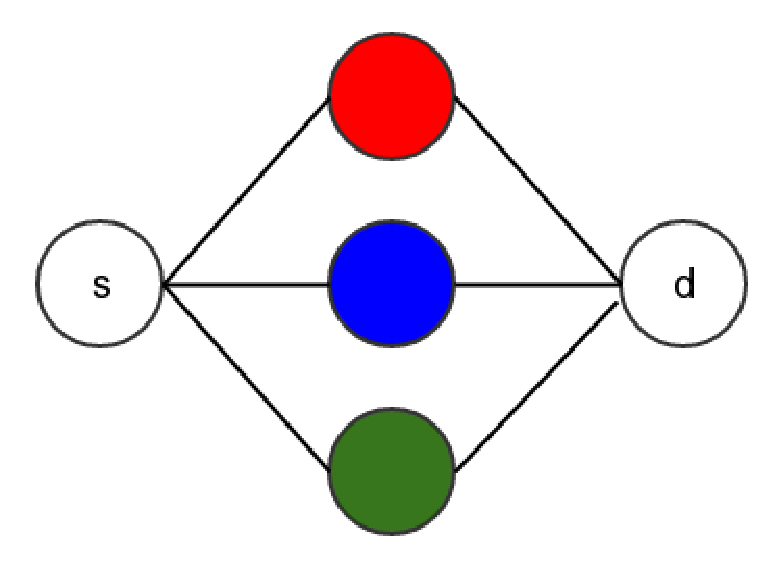
\includegraphics[width=0.7\columnwidth]{figures/color_topo.eps}
 	\caption{The switch topology $T$. All circles represent switches and all reachability policies are $s$ to $d$}
 	\label{fig:swtopo}
 \end{figure}
The solution to policy enforcement will be such that each reachability policy $r \in R$ from $s >> d$ will traverse through one of the colored switches $\{red$, $blue$, $green\}$. Color the vertices $R$ with the switch the path traverses through. If two vertices are connected by an edge in $I$, those flows would be isolated, and thus, will not have the same color. Thus, the problem reduces to finding a 3-graph coloring for the graph which is NP-complete. Thus, the enforcement of isolation policies is NP-complete. 
 
 In genral, k-coloring (for k > 2) is NP-complete and k-coloring problem reduces into a policy enforcement problem in a switch topology with k paths from source to destination, and thus, isolation policy enforcement is NP-complete. 
Similarly, The Hamiltonian Path problem can be reduced to an unordered waypoint policy, and thus, finding a path with unordered waypoints is NP-complete. The proof for this is omitted in this paper. 
 
% \subsection{Enforcement of Waypoint Policies}
% Given a undirected graph $G={V,E}$. Let us assume there exists an polynomial-time algorithm to compute the reachability paths satisfying the policies of the following types on the graph : \\
% \begin{itemize} 
% 	\item \textbf{P1} : $v_1 >> v_2 \Rightarrow$ There exists a path from $v_1$ to $v_2$ satisfying all input policies. A property of the path is that it does not have repeat a vertex (no forwarding loops).
% 	\item \textbf{P2} : $v_1 >> W >> v_2 \Rightarrow$ The path from $v_1$ to $v_2$  should pass through the vertices in the set $W$ in any order, without repeating a vertex.
% \end{itemize}
% \textbf{Reduction of Hamiltonian Cycle Problem} : Given a undirected graph $G={V,E}$, find $v \in V$ such that the degree of $v$ is the minimum in the graph (Will work for any vertex actually). If a Hamiltonian cycle is present in the graph, it will have the vertex $v$ in the cycle, and one of the edges from $v$.  \\
% Lets take a $n \in Neighbours(v)$. Let the input policies to our algorithm be : 
% \begin{itemize}
% 	\item \textbf{P4} : $v >> W >> n$ where $W = V - \{v,n\} $ 
% \end{itemize}
%P4 cimputes a simple path from $v$ to $n$ which passes through all the other vertices in the graph which is the Hamiltonian path problem. Since computing the Hamiltonian path is NP-hard, the problem of path computation for the waypoint policies as specified is NP-hard. 
\fi

\end{document}
